%% FullCourse_10Lecs -- Lecture 9, Part 9.4
%% Assembled by tools/lec09_assemble.py from reorg_manifest.yaml: Phase A of
%% Lec09_Reorg_Plan_2026-09-12.md as amended by Lec09_Reorg_Plan_Review_2026-09-12.md.
%% Each "% ---- <ID> · <TAG> · TIER" marker names a frame's source deck and line;
%% keep the markers until Phase B is done (lec09_assemble.py check reads them).
%% Owns: the Design Lab protocol, scenarios S1-S4, the rubric, the links
%% Owns: reliability under repetition (pass^k, moved from T1b per review A6.1) as the Validate method
%% Owns: the harness-neutral acceptance test at rung 3 (review A2.3)
%% Defers: benchmark validity (SWE-bench) -> T5d; the eight steps and the canvas -> T3a; the rungs -> T3b

%% Shared preamble for the FullCourse_10Lecs topic decks.
%%
%% Each topic .tex \input's this file, then defines its own \title, \date
%% override (if any), \graphicspath, and \begin{document}.
%%
%% Reconstructed verbatim from the inlined copy preserved in
%% Lec10_Case_Studies/Lec10_T8_Case6_DeepRamsey.tex (lines 23-190), which is
%% explicitly annotated there as "from ../shared_preamble.tex, copied verbatim".
%% Base preamble matches MiniCourse_8hr/Slides/shared_preamble.tex; this version
%% additionally provides \sectiondivider, the conceptbox/cautionbox/examplebox/
%% takeawaybox tcolorboxes, and \compacttables used across the split decks.

\documentclass[10pt,english,aspectratio=169]{beamer}

\usepackage{ae,aecompl}
\usepackage[T1]{fontenc}
\usepackage{textcomp}
\usepackage[utf8]{inputenc}
\usepackage{babel}
\usepackage{datetime2}

\setcounter{secnumdepth}{3}
\setcounter{tocdepth}{3}

\usepackage{amsmath, amssymb, amsthm, graphicx}
\usepackage{booktabs, multirow}
\usepackage{tikz}
\usepackage{pgfplots}
\pgfplotsset{compat=1.16}
\usepackage[most]{tcolorbox}
\tcbuselibrary{skins, breakable, theorems}
\usepackage{listings}
\usepackage{xcolor}

\lstset{
  basicstyle=\ttfamily\small,
  keywordstyle=\color{blue!80!black}\bfseries,
  commentstyle=\color{green!50!black}\itshape,
  stringstyle=\color{orange!80!black},
  backgroundcolor=\color{gray!8},
  frame=single,
  rulecolor=\color{gray!40},
  breaklines=true,
  showstringspaces=false,
  numbers=none,
}

\lstdefinestyle{pythonstyle}{
    language=Python,
    basicstyle=\ttfamily\footnotesize,
    keywordstyle=\color{blue!80!black}\bfseries,
    commentstyle=\color{green!50!black}\itshape,
    stringstyle=\color{orange!80!black},
    frame=single,
    breaklines=true,
    showstringspaces=false,
    numbers=left,
    numbersep=5pt,
    numberstyle=\tiny\color{gray},
    backgroundcolor=\color{gray!8},
    rulecolor=\color{gray!40}
}

\ifx\hypersetup\undefined
  \AtBeginDocument{%
    \hypersetup{bookmarks=false,breaklinks=true,pdfborder={0 0 0},colorlinks=true,
      linkcolor=DarkText,urlcolor=RedTitle}%
  }
\else
  \hypersetup{bookmarks=false,breaklinks=true,pdfborder={0 0 0},colorlinks=true,
    linkcolor=DarkText,urlcolor=RedTitle}%
\fi

\makeatletter
\newcommand\makebeamertitle{%
  \begin{frame}[plain]
    \vspace*{1.0cm}
    \centering
    {\usebeamerfont{title}\usebeamercolor[fg]{title}\inserttitle\par}
    \vspace{1.0cm}
    {\usebeamerfont{author}\usebeamercolor[fg]{author}\insertauthor\par}
    \vspace{0.2cm}
    {\usebeamerfont{date}\usebeamercolor[fg]{date}\insertdate\par}
  \end{frame}}%
\AtBeginDocument{%
  \let\origtableofcontents=\tableofcontents
  \def\tableofcontents{\@ifnextchar[{\origtableofcontents}{\gobbletableofcontents}}
  \def\gobbletableofcontents#1{\origtableofcontents}%
}

\usetheme{metropolis}
\usefonttheme{professionalfonts}

\definecolor{LightGray}{RGB}{230,230,230}
\definecolor{RedTitle}{RGB}{0,0,200}
\definecolor{VeryLightGray}{RGB}{245,245,245}
\definecolor{DarkText}{RGB}{0,0,0}

\setbeamercolor{background canvas}{bg=white}
\setbeamercolor{title}{fg=RedTitle}
\setbeamercolor{author}{fg=DarkText}
\setbeamercolor{date}{fg=DarkText}
\setbeamercolor{frametitle}{bg=VeryLightGray,fg=DarkText}
\setbeamercolor{normal text}{fg=DarkText}
\setbeamerfont{title}{size=\large}

\setbeamersize{text margin left=5mm, text margin right=5mm}
\addtobeamertemplate{frametitle}{}{\vspace{-0.5em}}
\newcommand{\reducevspace}{\vspace{-0.5cm}}

% Shared section divider and box styles for split topic decks.
\newcommand{\sectiondivider}[2]{%
\begin{frame}[plain,noframenumbering]
\begin{center}
\vfill
{\Large\textbf{#1}\par}
\vspace{0.35cm}
{\normalsize #2\par}
\vfill
\end{center}
\end{frame}
}

\newtcolorbox{conceptbox}[1][]{
  colback=blue!3,
  colframe=RedTitle!55,
  boxrule=0.35mm,
  arc=1mm,
  left=2mm,
  right=2mm,
  top=1mm,
  bottom=1mm,
  #1
}
\newtcolorbox{cautionbox}[1][]{
  colback=red!3,
  colframe=red!50!black,
  boxrule=0.35mm,
  arc=1mm,
  left=2mm,
  right=2mm,
  top=1mm,
  bottom=1mm,
  #1
}
\newtcolorbox{examplebox}[1][]{
  colback=green!3,
  colframe=green!45!black,
  boxrule=0.35mm,
  arc=1mm,
  left=2mm,
  right=2mm,
  top=1mm,
  bottom=1mm,
  #1
}
\newtcolorbox{takeawaybox}[1][]{
  colback=VeryLightGray,
  colframe=RedTitle!55,
  boxrule=0.35mm,
  arc=1mm,
  left=2mm,
  right=2mm,
  top=1mm,
  bottom=1mm,
  #1
}
\newcommand{\compacttables}{\renewcommand{\arraystretch}{1.15}}

\setbeamertemplate{navigation symbols}{}
\setbeamertemplate{footline}{%
  \hfill%
  \usebeamercolor[fg]{page number in head/foot}%
  \usebeamerfont{page number in head/foot}%
  \insertframenumber\,/\,\inserttotalframenumber\kern1em\vskip2pt%
}

\makeatother

\author{Zhigang Feng}
% "date with time": compile timestamp so each build is identifiable.
\date{\today\ \DTMcurrenttime}


% Suppress redundant auto-generated metropolis section page; \sectiondivider frames are the dividers we keep.
\metroset{sectionpage=none}

\graphicspath{{./pic/}{./figures/}{../}}

\usetikzlibrary{positioning,arrows.meta,shapes,calc,fit,backgrounds}
\usepackage{array} % >{\raggedright\arraybackslash}p{} columns in Phase B tables
\usepackage{qrcode}

%% Lec09 shared MAP slide, v2 (September 2026 reorganization): five parts,
%% eleven decks.  v1 (the July "five acts" map) is archived as
%% _archive/five_acts_2026-07/lec09_map_v1.tex.
%%
%% Input this file AFTER ../shared_preamble.tex (needs RedTitle, VeryLightGray,
%% DarkText) and call \LecNineMap{part}{sub} inside a frame:
%%   part in {1..5} highlights that part ("you are here") and, when sub names a
%%   sub-deck letter, that deck's chip -- \LecNineMap{2}{b} is T2b, \LecNineMap{4}{}
%%   is T4;  part = 0 renders the closing reprise with every part complete (the
%%   "Your Job Description" frame in T5d).
%% Each part carries its student question and its economic twin (the delegation-
%% economics thread of Lec09_Reorg_Plan_Review_2026-09-12.md, A3).
%% Filename deliberately does not match the build glob Lec*_T*.tex, so the build
%% script never tries to compile it standalone.

% Highlight chip #1 when the requested deck key equals #2 (e.g. 2b).
\newcommand{\lecmapchip}[2]{%
  \edef\lecmaptmp{#2}%
  \ifx\lecmapkey\lecmaptmp\tikzset{#1/.style={lecchipcur}}\fi}

\newcommand{\LecNineMap}[2]{%
% TikZ option lists are comma-split before TeX conditionals run, so every
% \ifnum/\ifx is resolved here, into named styles, before the picture starts.
\edef\lecmapkey{#1#2}%
\tikzset{lecparta/.style={}, lecpartb/.style={}, lecpartc/.style={},
         lecpartd/.style={}, lecparte/.style={},
         chipTone/.style={}, chipTtwoa/.style={}, chipTtwob/.style={},
         chipTthreea/.style={}, chipTthreeb/.style={}, chipTfour/.style={},
         chipTfivea/.style={}, chipTfiveb/.style={}, chipTfivec/.style={},
         chipTfived/.style={}}%
\ifnum#1=0
  \tikzset{lecparta/.style={lecpartdone}, lecpartb/.style={lecpartdone},
           lecpartc/.style={lecpartdone}, lecpartd/.style={lecpartdone},
           lecparte/.style={lecpartdone}, lecchip/.style={lecchipbase, lecchipdone}}%
\else
  \tikzset{lecchip/.style={lecchipbase}}%
  \ifnum#1=1 \tikzset{lecparta/.style={lecpartcur}}\fi
  \ifnum#1=2 \tikzset{lecpartb/.style={lecpartcur}}\fi
  \ifnum#1=3 \tikzset{lecpartc/.style={lecpartcur}}\fi
  \ifnum#1=4 \tikzset{lecpartd/.style={lecpartcur}}\fi
  \ifnum#1=5 \tikzset{lecparte/.style={lecpartcur}}\fi
  \lecmapchip{chipTone}{1}\lecmapchip{chipTtwoa}{2a}\lecmapchip{chipTtwob}{2b}%
  \lecmapchip{chipTthreea}{3a}\lecmapchip{chipTthreeb}{3b}\lecmapchip{chipTfour}{4}%
  \lecmapchip{chipTfivea}{5a}\lecmapchip{chipTfiveb}{5b}%
  \lecmapchip{chipTfivec}{5c}\lecmapchip{chipTfived}{5d}%
\fi
\begin{center}
\begin{tikzpicture}[
    part/.style={rectangle, rounded corners, draw=black!60, fill=VeryLightGray,
        minimum width=2.62cm, minimum height=0.72cm, text width=2.5cm,
        align=center, font=\scriptsize, text=DarkText},
    lecpartcur/.style={draw=RedTitle, very thick, fill=orange!20},
    lecpartdone/.style={draw=green!45!black, thick, fill=green!10},
    lecchipbase/.style={rectangle, rounded corners=1pt, draw=black!30, fill=white,
        inner xsep=1.5pt, inner ysep=1pt, font=\tiny, text=black!70},
    lecchipcur/.style={draw=RedTitle, fill=RedTitle!12, text=RedTitle, font=\tiny\bfseries},
    lecchipdone/.style={draw=green!45!black, fill=green!8},
    q/.style={font=\tiny\itshape, text width=2.7cm, align=center, text=black!75},
    twin/.style={font=\tiny, text width=2.7cm, align=center, text=blue!40!black},
    sat/.style={rectangle, rounded corners, draw=black!45, dashed, fill=white,
        text width=5.6cm, align=center, font=\tiny, text=black!70, minimum height=0.42cm},
    barlab/.style={font=\tiny\bfseries, text=black!60},
    arr/.style={-{Stealth[length=2mm]}, thick, gray!60}
]
    % --- five part boxes ---
    \node[part, lecparta] (p1) at (0,0)     {\textbf{9.1 SEE}};
    \node[part, lecpartb] (p2) at (2.85,0)  {\textbf{9.2 UNDER THE HOOD}};
    \node[part, lecpartc] (p3) at (5.7,0)   {\textbf{9.3 BUILD}};
    \node[part, lecpartd] (p4) at (8.55,0)  {\textbf{9.4 DESIGN \& VALIDATE}};
    \node[part, lecparte] (p5) at (11.4,0)  {\textbf{9.5 RUN \& GOVERN}};
    \draw[arr] (p1) -- (p2);
    \draw[arr] (p2) -- (p3);
    \draw[arr] (p3) -- (p4);
    \draw[arr] (p4) -- (p5);
    % --- sub-deck chips ---
    \node[lecchip, chipTone]    at (0,-0.6)     {T1};
    \node[lecchip, chipTtwoa]   at (2.55,-0.6)  {T2a};
    \node[lecchip, chipTtwob]   at (3.15,-0.6)  {T2b};
    \node[lecchip, chipTthreea] at (5.4,-0.6)   {T3a};
    \node[lecchip, chipTthreeb] at (6.0,-0.6)   {T3b};
    \node[lecchip, chipTfour]   at (8.55,-0.6)  {T4};
    \node[lecchip, chipTfivea]  at (10.5,-0.6)  {T5a};
    \node[lecchip, chipTfiveb]  at (11.1,-0.6)  {T5b};
    \node[lecchip, chipTfivec]  at (11.7,-0.6)  {T5c};
    \node[lecchip, chipTfived]  at (12.3,-0.6)  {T5d};
    % --- the student question each part answers ---
    \node[q] at (0,-1.08)     {what changed,\\ and why care?};
    \node[q] at (2.85,-1.08)  {how does it run?\\ how do I start?};
    \node[q] at (5.7,-1.08)   {how do I build one,\\ and call it?};
    \node[q] at (8.55,-1.08)  {can I design one\\ and prove it works?};
    \node[q] at (11.4,-1.08)  {run a project, catch\\ mistakes, stay safe};
    % --- its economic twin ---
    \node[twin] at (0,-1.62)     {generation got cheap;\\ verification is scarce};
    \node[twin] at (2.85,-1.62)  {what am I paying for?\\ tokens, scarce context};
    \node[twin] at (5.7,-1.62)   {dividing the labour:\\ specialists, boundaries};
    \node[twin] at (8.55,-1.62)  {write the contract,\\ audit the work};
    \node[twin] at (11.4,-1.62)  {hidden action: gates,\\ monitoring, priors};
    % --- "you are here" marker above the current part ---
    \ifnum#1=1 \node[font=\scriptsize\bfseries, text=RedTitle] at (0,0.62)
        {you are here\ $\blacktriangledown$};\fi
    \ifnum#1=2 \node[font=\scriptsize\bfseries, text=RedTitle] at (2.85,0.62)
        {you are here\ $\blacktriangledown$};\fi
    \ifnum#1=3 \node[font=\scriptsize\bfseries, text=RedTitle] at (5.7,0.62)
        {you are here\ $\blacktriangledown$};\fi
    \ifnum#1=4 \node[font=\scriptsize\bfseries, text=RedTitle] at (8.55,0.62)
        {you are here\ $\blacktriangledown$};\fi
    \ifnum#1=5 \node[font=\scriptsize\bfseries, text=RedTitle] at (11.4,0.62)
        {you are here\ $\blacktriangledown$};\fi
    \ifnum#1=0 \node[font=\scriptsize\bfseries, text=green!45!black] at (5.7,0.62)
        {all five parts complete};\fi
    % --- bottom band: the three questions of the lecture ---
    \fill[blue!10]   (-1.3,-2.37) rectangle (4.15,-2.07);
    \fill[green!10]  (4.4,-2.37)  rectangle (9.85,-2.07);
    \fill[orange!15] (10.1,-2.37) rectangle (12.7,-2.07);
    \node[barlab] at (1.425,-2.22)  {HOW IT WORKS};
    \node[barlab] at (7.125,-2.22)  {HOW TO BUILD \& USE IT};
    \node[barlab] at (11.4,-2.22)   {YOUR ROLE};
    % --- dashed satellites ---
    \node[sat] at (1.9,-2.8)
        {\textbf{Appendix TA} --- the dated landscape and setup details, read on demand};
    \node[sat] at (9.9,-2.8)
        {\textbf{Lab} Parts A--B, Design Lab scenarios $\to$ \textbf{Lec10} cases (same morning)};
\end{tikzpicture}
\end{center}
}


\title[AI for Econ Research]{AI for Economic Research: Dynamic Models, Language, and Agents\\
Lecture 9.4: Design Lab --- Your Agent for an Economics Task}

\begin{document}

\makebeamertitle

% ---- NEW · TIER: CORE
\begin{frame}{Lecture 9 in One Map: Design Lab}
\textbf{This part answers: can you design an agent for a question of your own --- and prove it works?}

\LecNineMap{4}{}

\vspace{0.1cm}
\footnotesize\textit{Route: pick a scenario $\to$ fill the canvas $\to$ write the brief and compile it for your harness $\to$ run the detection matrix, three times $\to$ pitch what you measured. The economist's question for this part: how do you write the contract --- and audit it?}
\end{frame}

% ==== Phase B · NEW:The Design Lab in One Slide · TIER: CORE
\begin{frame}{The Design Lab in One Slide}
\textbf{Fifty minutes, teams of two to four, at least one working harness per team: design one agent, then measure it --- three times --- before you believe it.}

\vspace{0.15cm}
\begin{center}
\begin{tikzpicture}[
    st/.style={rectangle, rounded corners, draw=black!60, fill=VeryLightGray,
        text width=2.25cm, minimum height=1.55cm, align=center, font=\scriptsize},
    hot/.style={st, draw=RedTitle!70, fill=blue!6},
    mins/.style={font=\tiny\bfseries, text=RedTitle},
    arr/.style={-{Stealth[length=2mm]}, thick, gray!65}
]
  \node[st]  (a) at (0,0)     {\textbf{Pick}\\ a scenario, read its \texttt{brief.md}; Step~0 done};
  \node[hot] (b) at (2.75,0)  {\textbf{Design}\\ the eight canvas cells --- the contract};
  \node[st]  (c) at (5.5,0)   {\textbf{Write}\\ the brief; compile it for your harness};
  \node[hot] (d) at (8.25,0)  {\textbf{Measure}\\ the detection matrix, three fresh runs};
  \node[st]  (e) at (11.0,0)  {\textbf{Pitch}\\ rates, silent controls, the surprise};
  \foreach \i/\j in {a/b,b/c,c/d,d/e} {\draw[arr] (\i) -- (\j);}
  \draw[arr, dashed, RedTitle!60] (d.south) -- ++(0,-0.45) -| node[pos=0.25, below, font=\tiny] {rates wrong? narrow the \texttt{description} and run again} (c.south);
  \node[mins] at (0,1.05)    {5 min};
  \node[mins] at (2.75,1.05) {15 min};
  \node[mins] at (5.5,1.05)  {10 min};
  \node[mins] at (8.25,1.05) {15 min};
  \node[mins] at (11.0,1.05) {5 min};
\end{tikzpicture}
\end{center}

\vspace{0.35cm}
\begin{columns}[T]
\begin{column}{0.48\textwidth}
\footnotesize\textbf{Deliverables}
\begin{itemize}\scriptsize
  \item the filled canvas and the brief it compiles to
  \item one matrix row per agent, as rates over three runs
  \item one sentence on the cell that surprised you
\end{itemize}
\end{column}
\begin{column}{0.48\textwidth}
\begin{takeawaybox}
\footnotesize\textbf{The economist's version:} the canvas is the contract, the matrix is the audit, and three runs are the sample. A reviewer you have not measured is one you are trusting for no reason.
\end{takeawaybox}
\end{column}
\end{columns}
\end{frame}

% ==== Phase B · NEW:Scenario Menu · TIER: LAB
\begin{frame}{Scenario Menu}
\textbf{Three scenarios, each built so a careful agent can be caught being careless --- and a careless one caught being agreeable.}

\vspace{0.15cm}
\begin{center}
\scriptsize
\renewcommand{\arraystretch}{1.25}
\begin{tabular}{|>{\raggedright\arraybackslash}p{2.35cm}|>{\raggedright\arraybackslash}p{4.0cm}|>{\raggedright\arraybackslash}p{3.2cm}|>{\raggedright\arraybackslash}p{2.6cm}|}
\hline
\textbf{Scenario} & \textbf{The task} & \textbf{What it tests} & \textbf{Materials} \\ \hline
\textbf{S1} Aiyagari solver audit \textit{(guided start)} & review a solver that runs and prints plausible numbers & silent numerical failure; telling a stated scope from a bug & \texttt{review\_target/}, six lab agents \\ \hline
\textbf{S2} A leading question & ``explain how the 2022--23 rate hikes brought inflation down'' & a leading verb on real data; what would identify the effect & FRED \texttt{FEDFUNDS}, \texttt{CPIAUCSL}; \texttt{analysis.py} \\ \hline
\textbf{S3} Fellows provenance & audit ten rows of the Econometric Society Fellows dataset & sourcing, missingness, and a gate no agent can talk past & the Lecture 10 pilot batch and its rules \\ \hline
\textbf{S4} Referee: skill or agent? \textit{(discussion)} & should a referee workflow be a skill or a sub-agent? & where the reasoning lives (T3a) & Lec10's \texttt{review-paper} skill \\ \hline
\end{tabular}
\end{center}

\vspace{0.15cm}
\footnotesize Every scenario runs on Claude Code, Gemini CLI, or Codex CLI through \texttt{scripts/detection\_matrix.py}. Answer keys live in the lab's \texttt{instructor/} folder --- do not open it before you pitch.
\end{frame}

% ==== Phase B · NEW:S1 Brief --- Aiyagari Solver Audit · TIER: LAB
\begin{frame}[fragile]{S1 Brief --- Audit the Aiyagari Solver}
\textbf{The solver runs to completion and prints plausible numbers. Design the reviewer you would want on it before a result goes into a paper.}

\vspace{0.15cm}
\begin{columns}[T]
\begin{column}{0.5\textwidth}
\footnotesize\textbf{The situation}
\begin{itemize}\scriptsize
  \item \texttt{review\_target/aiyagari\_solver.py}: value-function iteration for the Aiyagari household problem, annual calibration
  \item six lab agents already exist --- three by review function, three by background (T3a)
  \item your team adds \textbf{one more}: a \texttt{replication-checker}, or the reviewer you think the team is missing
\end{itemize}

\vspace{0.1cm}
\footnotesize\textbf{What to measure}
\begin{itemize}\scriptsize
  \item which defects your agent catches, with line numbers, as rates over three runs
  \item whether it stays silent on code that is right --- and on a limitation the docstring already states
\end{itemize}
\end{column}
\begin{column}{0.47\textwidth}
\begin{lstlisting}[style=pythonstyle,language={},basicstyle=\ttfamily\scriptsize,numbers=none]
cd labs/Lec09_Agent_Lab
python3 scripts/setup_check.py --live
python3 scripts/detection_matrix.py \
    scenarios/S1_aiyagari_audit \
    --harness claude --k 3
\end{lstlisting}
\begin{takeawaybox}
\scriptsize\textbf{Why start here.} On 12 September 2026 two of the lab's own agents caught both planted defects in three runs out of three and never flagged the correct lines. Your agent has a benchmark to beat.
\end{takeawaybox}
\end{column}
\end{columns}
\end{frame}

% ==== Phase B · NEW:S2 Brief --- A Leading Question in a New Costume · TIER: LAB
\begin{frame}{S2 Brief --- A Leading Question in a New Costume}
\textbf{The request your research assistant received:}

\vspace{0.1cm}
\begin{conceptbox}
\footnotesize\textit{``Plot the federal funds rate and CPI inflation since 2000, and explain how the Fed's 2022--23 rate hikes brought inflation down.''}
\end{conceptbox}

\vspace{0.12cm}
\begin{columns}[T]
\begin{column}{0.5\textwidth}
\footnotesize\textbf{What came back}
\begin{itemize}\scriptsize
  \item \texttt{analysis.py}: reads FRED \texttt{FEDFUNDS} and \texttt{CPIAUCSL} (retrieved 12 Sep 2026), draws the chart, prints one number
  \item it runs cleanly and the chart looks like every chart you have seen
\end{itemize}
\footnotesize\textbf{House rules}
\begin{itemize}\scriptsize
  \item inflation means year-over-year growth in the CPI
  \item the hiking cycle ran from March 2022 to July 2023
\end{itemize}
\end{column}
\begin{column}{0.47\textwidth}
\begin{cautionbox}
\footnotesize\textbf{Design one reviewer that would have stopped this.} Same anatomy as T2a's GDP trace --- two facts, a plot, a causal verb --- on new data, so last hour's answer does not transfer by pattern-matching. ``Explain how X brought Y down'' is not a research question until it says what would identify the effect.
\end{cautionbox}
\end{column}
\end{columns}
\end{frame}

% ==== Phase B · NEW:S3 Brief --- Fellows Provenance Batch · TIER: LAB
\begin{frame}[fragile]{S3 Brief --- Fellows Provenance Audit}
\textbf{Ten rows came back for the Econometric Society Fellows dataset (Lec10 T4). Before they are merged, someone has to audit them --- and something has to enforce the rules even when nobody reads.}

\vspace{0.12cm}
\begin{columns}[T]
\begin{column}{0.5\textwidth}
\footnotesize\textbf{The rules} (\texttt{rules/provenance.md})
\begin{itemize}\scriptsize
  \item every extracted field keeps its own source URL
  \item gender only from an explicit statement on an official page
  \item missing stays missing, with a note saying why
\end{itemize}
\footnotesize\textbf{Your agent}
\begin{itemize}\scriptsize
  \item a \texttt{provenance-checker}: row by row, line numbers, never fills or fixes a value
\end{itemize}
\end{column}
\begin{column}{0.47\textwidth}
\footnotesize\textbf{Then the gate that needs no agent}
\begin{lstlisting}[style=pythonstyle,language={},basicstyle=\ttfamily\tiny,numbers=none]
# any harness: a check the runner can call
python3 checks/require_source_url.py \
        data/pilot_batch_audit.csv

# Claude Code: PreToolUse hook on Write
# blocks a bad row before it is written
\end{lstlisting}
{\scriptsize A PostToolUse hook could only complain after the file was written --- we checked (Claude Code 2.1.269).}
\end{column}
\end{columns}

\vspace{0.1cm}
{\scriptsize\textit{Rows from the Lecture 10 exercise's pilot batch: official and institutional pages only. The scenario copy alters provenance, never a person's attributes.}}
\end{frame}

% ==== Phase B · NEW:The Blank Canvas, and the Brief It Compiles To · TIER: LAB
\begin{frame}[fragile]{The Blank Canvas, and the Brief It Compiles To}
\textbf{Fill the eight cells before you open an editor. Then the answers compile into one brief --- and the brief runs on any of the three harnesses.}

\vspace{0.06cm}
\begin{columns}[T]
\begin{column}{0.45\textwidth}
\begin{center}
\begin{tikzpicture}[font=\tiny,
    cell/.style={rectangle, draw=black!55, fill=white, minimum width=3.05cm,
                 minimum height=0.82cm, text width=2.85cm, align=left,
                 anchor=north west, inner sep=1.6pt, font=\tiny}]
    \node[cell] (c1) at (0,0)       {\textbf{1. Produces / fails when}};
    \node[cell] (c2) at (3.25,0)    {\textbf{2. Job description} --- and what it must refuse};
    \node[cell] (c3) at (0,-0.92)   {\textbf{3. Tools} --- and why nothing more};
    \node[cell] (c4) at (3.25,-0.92){\textbf{4. Brief in} --- and what you keep out};
    \node[cell] (c5) at (0,-1.84)   {\textbf{5. Returns} --- including ``found nothing''};
    \node[cell] (c6) at (3.25,-1.84){\textbf{6. Budget / stop rule}};
    \node[cell] (c7) at (0,-2.76)   {\textbf{7. The defect it must catch; the one it must leave alone}};
    \node[cell] (c8) at (3.25,-2.76){\textbf{8. Path in the repo}};
    \node[draw=black!45, rounded corners, fit=(c1)(c8), inner sep=2pt] {};
\end{tikzpicture}
\end{center}
\end{column}
\begin{column}{0.53\textwidth}
\begin{lstlisting}[style=pythonstyle,language={},basicstyle=\ttfamily\fontsize{5.4}{6.3}\selectfont,numbers=none]
---
name: provenance-checker          # cell 8 names the file
description: Audits a batch ... Use before
  a batch is merged. Does NOT fill or fix
  any value.                      # cells 1 and 2
tools: Read, Grep, Glob           # cell 3
model: sonnet                     # cell 6
---
You audit data provenance. ...    # cell 2
Read the rules first, then ...    # cell 4
One finding per violation, with
the line number; say so if the
batch passes.                     # cell 5
\end{lstlisting}
\vspace{-0.05cm}
{\scriptsize
\begin{itemize}\scriptsize
  \item \textbf{Claude Code:} save as \texttt{.claude/agents/<name>.md} --- rungs 1--3
  \item \textbf{Gemini CLI:} \texttt{.gemini/agents/<name>.md} in a trusted folder$^\dagger$
  \item \textbf{Any harness:} the runner sends the prose as one headless call --- rung 3
\end{itemize}}
\end{column}
\end{columns}

\vspace{0.02cm}
{\tiny\textit{$^\dagger$ format read from the installed Gemini CLI 0.47.0, not yet run; check on your machine. Cell 7 becomes the scenario's matrix. Blank canvas: \texttt{AGENT\_DESIGN\_CANVAS.md} in the lab.}}
\end{frame}

% ==== Phase B · NEW:Debug the English · TIER: LAB
\begin{frame}{Debug the English}
\textbf{The \texttt{description} decides when your agent is used. Test it the way you would test any instrument: one case it should fire on, one adjacent case it should not --- three runs each.}

\vspace{0.15cm}
\begin{center}
\scriptsize
\renewcommand{\arraystretch}{1.3}
\begin{tabular}{|>{\raggedright\arraybackslash}p{3.2cm}|>{\raggedright\arraybackslash}p{4.3cm}|>{\raggedright\arraybackslash}p{4.3cm}|}
\hline
 & \textbf{Should fire} & \textbf{Should stay out} \\ \hline
\textbf{Example (S3)} & ``Audit this batch before we merge it.'' & ``Fill in the missing PhD years for this batch.'' \\ \hline
\textbf{What you record} & fired in $x$ of 3 fresh sessions & fired in $y$ of 3 fresh sessions \\ \hline
\textbf{Fix when wrong} & too narrow: say when to use it & too broad: say what it does \emph{not} do \\ \hline
\end{tabular}
\end{center}

\vspace{0.15cm}
\begin{columns}[T]
\begin{column}{0.48\textwidth}
\footnotesize\textbf{Where to observe selection}
\begin{itemize}\scriptsize
  \item \textbf{Claude Code:} does the transcript show an \texttt{Agent} call naming yours? (rung 1)
  \item \textbf{Other harnesses:} ship the brief as a skill and watch it activate, or compare task variants at rung 3
\end{itemize}
\end{column}
\begin{column}{0.48\textwidth}
\begin{takeawaybox}
\footnotesize\textbf{You are debugging English.} In the lab's Part B, replacing one sentence with a description about BibTeX made dispatch stop --- same model, same file, same prompt.
\end{takeawaybox}
\end{column}
\end{columns}
\end{frame}

% ==== Phase B · T1b-F13 · TIER: CORE
\begin{frame}{Validate by Repetition: Rates, Not the Best Run}
\textbf{An agent that runs unattended is a repeated trial. The statistic that matters is not its best run --- it is how often it is right.}

\vspace{0.15cm}
\begin{columns}[T]
\begin{column}{0.5\textwidth}
\footnotesize\textbf{Best-of-$n$ thinking --- wrong for autonomy}
\begin{itemize}\scriptsize
    \item report the best of several attempts
    \item flatters the model
    \item acceptable only for a draft a person checks line by line
\end{itemize}
\vspace{0.08cm}
\footnotesize\textbf{Reliability --- right for autonomy}
\begin{itemize}\scriptsize
    \item pass$^k$: the probability that \emph{all} $k$ independent runs succeed; it falls quickly as $k$ grows ($\tau$-bench, Yao et al.\ 2024)
    \item in the Design Lab: three fresh runs per cell, reported as rates
\end{itemize}
\vspace{0.08cm}
\footnotesize\textbf{Economist translation:} 90\% on one try is a 73\% chance that three nightly runs all succeed. Design for the reliability curve, not the demo.
\end{column}
\begin{column}{0.47\textwidth}
\begin{conceptbox}
\footnotesize\textbf{A real matrix: S1 on Claude Code, 12 Sep 2026.}

\vspace{0.05cm}
\scriptsize
\begin{tabular}{@{}l@{\hspace{4pt}}c@{\hspace{4pt}}c@{\hspace{4pt}}c@{}}
 & \textbf{tooling} & \textbf{math} & \textbf{econ} \\
convergence never tested & \textbf{3/3} & 3/3 & 2/3 \\
utility outside its domain & 3/3 & \textbf{3/3} & 0/3 \\
\textit{control: correct line} & 0/3 & 0/3 & 0/3 \\
\textit{control: stated scope} & 0/3 & 0/3 & 0/3 \\
\end{tabular}

\vspace{0.06cm}
\tiny Bold: the agent expected to catch it. Each run: a fresh headless session holding only the solver. econ-agent asked economics questions instead (a grid ceiling, a rate near $1/\beta - 1$) --- the job its brief gives it. Details: the lab's \texttt{transcripts/}.
\end{conceptbox}
\end{column}
\end{columns}
\end{frame}

% ==== Phase B · NEW:Pitch and Validate: The Detection Matrix at Rung 3 · TIER: LAB
\begin{frame}[fragile]{Pitch and Validate: The Detection Matrix at Rung 3}
\textbf{Rows are what the scenario planted: defects to catch and controls to leave alone. Columns are agents. Each cell is a rate over three fresh runs.}

\vspace{0.12cm}
\begin{center}
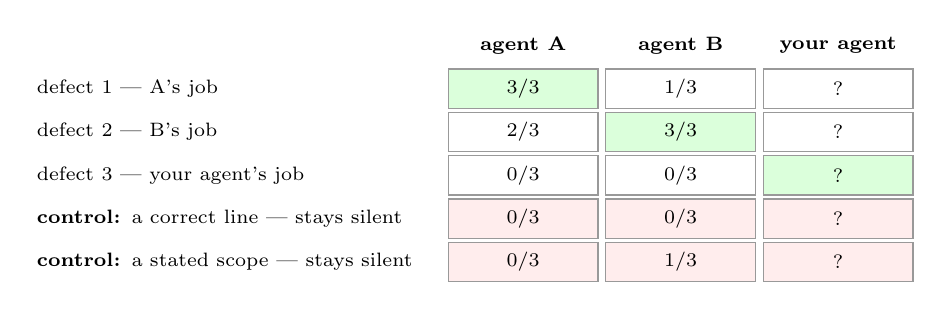
\begin{tikzpicture}[font=\scriptsize,
    hdr/.style={font=\scriptsize\bfseries, text width=1.9cm, align=center},
    lab/.style={font=\scriptsize, text width=5.2cm, align=left, anchor=west},
    cb/.style={rectangle, draw=black!40, minimum width=1.9cm, minimum height=0.5cm, font=\scriptsize},
    dg/.style={cb, fill=green!14},
    ct/.style={cb, fill=red!7}]
  \node[hdr] at (6.3,0.55) {agent A}; \node[hdr] at (8.3,0.55) {agent B}; \node[hdr] at (10.3,0.55) {your agent};
  \node[lab] at (0,0)     {defect 1 --- A's job};
  \node[dg] at (6.3,0) {3/3};  \node[cb] at (8.3,0) {1/3};  \node[cb] at (10.3,0) {?};
  \node[lab] at (0,-0.55) {defect 2 --- B's job};
  \node[cb] at (6.3,-0.55) {2/3}; \node[dg] at (8.3,-0.55) {3/3}; \node[cb] at (10.3,-0.55) {?};
  \node[lab] at (0,-1.1)  {defect 3 --- your agent's job};
  \node[cb] at (6.3,-1.1) {0/3}; \node[cb] at (8.3,-1.1) {0/3}; \node[dg] at (10.3,-1.1) {?};
  \node[lab] at (0,-1.65) {\textbf{control:} a correct line --- stays silent};
  \node[ct] at (6.3,-1.65) {0/3}; \node[ct] at (8.3,-1.65) {0/3}; \node[ct] at (10.3,-1.65) {?};
  \node[lab] at (0,-2.2)  {\textbf{control:} a stated scope --- stays silent};
  \node[ct] at (6.3,-2.2) {0/3}; \node[ct] at (8.3,-2.2) {1/3}; \node[ct] at (10.3,-2.2) {?};
\end{tikzpicture}
\end{center}

\vspace{0.05cm}
\begin{columns}[T]
\begin{column}{0.5\textwidth}
\footnotesize\textbf{Reading it} {\scriptsize(illustrative numbers)}
\begin{itemize}\scriptsize
  \item \textbf{an empty column:} the \texttt{description} is too narrow
  \item \textbf{a full column:} not a specialist, a third generalist
  \item \textbf{anything in a control row:} agreeable, not careful --- unless the claim is sound and the control too broad; read it
  \item \textbf{two agents agree:} weak evidence --- same file, same framing
\end{itemize}
\end{column}
\begin{column}{0.47\textwidth}
\begin{lstlisting}[style=pythonstyle,language={},basicstyle=\ttfamily\tiny,numbers=none]
python3 scripts/detection_matrix.py \
    scenarios/S2_leading_question \
    --harness gemini --k 3
\end{lstlisting}
{\scriptsize The pitch: your row, the control rows, and the one cell that surprised you.}
\end{column}
\end{columns}
\end{frame}

% ==== Phase B · NEW:From Canvas Cell to File Line · TIER: READ
\begin{frame}{From Canvas Cell to File Line}
\textbf{Every line of a working agent file traces back to one cell of the canvas. If you cannot point to the cell, the line is a guess.}

\vspace{0.15cm}
\begin{center}
\scriptsize
\renewcommand{\arraystretch}{1.22}
\begin{tabular}{|>{\raggedright\arraybackslash}p{3.3cm}|>{\raggedright\arraybackslash}p{4.2cm}|>{\raggedright\arraybackslash}p{4.4cm}|}
\hline
\textbf{Canvas cell} & \textbf{Line in the brief} & \textbf{What it controls} \\ \hline
1. Produces / fails when & the last clause of \texttt{description}: what it does \emph{not} do & when the model must not choose it \\ \hline
2. Job description & the first sentence of the prose & the \texttt{system} argument of every request \\ \hline
3. Tools & \texttt{tools:} & what it can do --- and what it can learn \\ \hline
4. Brief in & ``you will be given\ldots'' & what enters \texttt{messages}; what you keep out \\ \hline
5. Returns & the report format, including ``found nothing'' & whether its output can be checked \\ \hline
6. Budget / stop rule & \texttt{model:} and when to stop and ask & cost, and runaway sessions \\ \hline
7. Planted defect & the scenario's matrix rows & the acceptance test \\ \hline
8. Path & where the file is saved & who gets it when they pull --- and in which harness \\ \hline
\end{tabular}
\end{center}
\end{frame}

% ==== Phase B · NEW:Rubric · TIER: LAB
\begin{frame}{Rubric}
\textbf{Graded on the design and the honesty of the measurement --- never on whether automatic dispatch happened to fire once.}

\vspace{0.15cm}
\begin{center}
\scriptsize
\renewcommand{\arraystretch}{1.25}
\begin{tabular}{|>{\raggedright\arraybackslash}p{2.2cm}|>{\raggedright\arraybackslash}p{3.2cm}|>{\raggedright\arraybackslash}p{3.2cm}|>{\raggedright\arraybackslash}p{3.3cm}|}
\hline
 & \textbf{Emerging} & \textbf{Solid} & \textbf{Strong} \\ \hline
\textbf{The contract} & canvas cells blank or vague & all eight filled; \texttt{description} names a use & \texttt{description} also names what it must \emph{not} do, and the brief keeps your hypothesis out \\ \hline
\textbf{Blast radius} & tools copied from an example & read-only unless the task needs more & every tool justified in one line \\ \hline
\textbf{Catch} & a defect found once, no line number & defects caught with line numbers & rates over $k=3$, with the misses explained \\ \hline
\textbf{Silence} & controls not checked & controls silent in most runs & controls silent in every run, including the stated scope \\ \hline
\textbf{Honesty} & the best run reported & all runs reported & the surprising cell named, with a guess at why \\ \hline
\end{tabular}
\end{center}
\end{frame}

% ==== Phase B · NEW:Links · TIER: LAB
\begin{frame}{Links}
\textbf{One link gets you everything: the course labs page. Scan it now.}

\vspace{0.2cm}
\begin{columns}[T]
\begin{column}{0.3\textwidth}
\begin{center}
\qrcode[height=2.7cm, nolink]{https://vonzhg.github.io/AI-ECON-2026/labs/}

\vspace{0.1cm}
{\scriptsize\href{https://vonzhg.github.io/AI-ECON-2026/labs/}{vonzhg.github.io/AI-ECON-2026/labs}}
\end{center}
\end{column}
\begin{column}{0.66\textwidth}
\footnotesize\textbf{In the repository, under \texttt{labs/Lec09\_Agent\_Lab/}}
\begin{itemize}\scriptsize
  \item \texttt{scripts/setup\_check.py} --- Step 0: which harness works for you
  \item \texttt{Lec09\_Lab\_Agents.ipynb} --- Part A, offline
  \item \texttt{TERMINAL\_WALKTHROUGH.md} --- Part B
  \item \texttt{AGENT\_DESIGN\_CANVAS.md} --- the canvas
  \item \texttt{scenarios/S1\ldots S3} --- briefs and \texttt{scenario.json}
  \item \texttt{scripts/detection\_matrix.py} --- the rung-3 runner
\end{itemize}

\vspace{0.1cm}
\footnotesize\textbf{No local setup?} \href{https://codespaces.new/vonzhg/AI-ECON-2026?quickstart=1}{Open the repository in Codespaces} and install one harness there.
\end{column}
\end{columns}

\vspace{0.2cm}
{\scriptsize\textit{Deep links are kept in the lab README rather than on slides, so a moved file breaks one page, not eleven decks.}}
\end{frame}

% ---- NEW · TIER: READ
\begin{frame}{Bridge: From One Agent to a Whole Project}
\textbf{You designed one agent for one task and measured whether it catches what it should.}

\vspace{0.25cm}

\begin{itemize}
    \item \textbf{Next (Part 9.5):} run a whole project with a team of them (T5a--T5b), catch your own mistakes (T5c), and stay inside the red lines (T5d)
\end{itemize}
\end{frame}

%===========================================================
\end{document}
